\documentclass[letterpaper, 10 pt, conference]{ieeeconf}  % Comment this line out if you need a4paper

%\documentclass[a4paper, 10pt, conference]{ieeeconf}      % Use this line for a4 paper

\IEEEoverridecommandlockouts                              % This command is only needed if 
                                                          % you want to use the \thanks command

\overrideIEEEmargins                                      % Needed to meet printer requirements.




% The following packages can be found on http:\\www.ctan.org
\usepackage{graphics} % for pdf, bitmapped graphics files
\usepackage{epsfig} % for postscript graphics files
% \usepackage{times}
% \usepackage{newtxtext,newtxmath} % Times-like text and math fonts

\usepackage{mathptmx} % assumes new font selection scheme installed
\usepackage{times} % assumes new font selection scheme installed
\usepackage{amsmath} % assumes amsmath package installed
\usepackage{amssymb}  % assumes amsmath package installed
% \usepackage[utf8]{inputenc}

\usepackage{cite} % Use cite.sty for numerical citation management
\usepackage[bookmarks=true]{hyperref} % Use hyperref for other links
% \usepackage{hyperref} % Use hyperref for other links

\usepackage{tikz}
\usepackage{float}
\usepackage{svg}
\usepackage{bm}

\tikzstyle{block} = [rectangle, minimum width=2cm, minimum height=1cm,text centered, draw=black]
\tikzstyle{block_1} = [rectangle, minimum width=2cm, minimum height=1cm,text centered, draw=black, fill=blue!5]
\tikzstyle{block_2} = [rectangle, minimum width=2cm, minimum height=1cm,text centered, draw=black, fill=red!5]
\tikzstyle{arrow} = [thick,->,>=stealth]
\tikzstyle{arrow_2} = [very thick,->,>=stealth]
\tikzstyle{arrow_3} = [thick,->,>=stealth,dashed]
\tikzstyle{pfr} = [cylinder, draw, minimum height=4cm, minimum width=1cm, shape aspect=1, shape border rotate=180]
\usetikzlibrary{shapes.geometric}


% Override the fake natbib command to allow cite.sty and hyperref to work together
\makeatletter
\let\NAT@parse\undefined
\makeatletter

\title{\LARGE \bf
Model Predictive Control of Axial Dispersion Tubular Reactors\\ with Recycle: Addressing State-delay through Transport PDEs*
}


\author{Behrad Moadeli and Stevan Dubljevic$^{1}$% <-this % stops a space
\thanks{*This work was not supported by any organization}% <-this % stops a space
\thanks{$^{1}$Behrad Moadeli and Stevan Dubljevic are with the Department of Chemical and Materials Engineering,
         University of Alberta, Edmonton, AB, Canada T6G 1H9
        {\tt\small moadeli@ualberta.ca}, {\tt\small stevan.dubljevic@ualberta.ca}}%
}


\begin{document}



\maketitle
\thispagestyle{empty}
\pagestyle{empty}


%%%%%%%%%%%%%%%%%%%%%%%%%%%%%%%%%%%%%%%%%%%%%%%%%%%%%%%%%%%%%%%%%%%%%%%%%%%%%%%%
\begin{abstract}

        This paper presents the model predictive control of an axial tubular reactor with a recycle stream, where the intrinsic time delay imposed by the recycle stream—often overlooked in prior studies—is modeled as a transport PDE. This leads to a boundary-controlled system of coupled parabolic and hyperbolic PDEs under Danckwerts boundary conditions, ideal for this reactor type. A discrete-time linear model predictive controller is designed to stabilize the system. Utilizing Caley-Tustin time discretization along with the late lumping approach, the system's infinite-dimensional characteristics are preserved with no need for model reduction or spatial approximation. Numerical simulations demonstrate the controller’s effectiveness in stabilizing an unstable system while satisfying input constraints.

\end{abstract}

\section{Introduction}

Many processes in the chemical and petrochemical sectors involve states that evolve over space and time, commonly represented by partial differential equations (PDEs) as distributed parameter systems (DPS) \cite{ray1981advanced}. The infinite-dimensional nature of DPSs presents specific challenges in control and estimation, making this a prominent area of research. Two main methods are often applied to control DPSs: \textit{Early Lumping} and \textit{Late Lumping}. Early Lumping reduces the system to a finite-dimensional approximation through spatial discretization early in the modeling stage, allowing for the application of standard control techniques \cite{davison1976robust}. However, this method can lead to inaccuracies due to mismatches between the reduced model and the original system dynamics \cite{moghadam2012infinite}. Late Lumping, by contrast, preserves the system’s infinite-dimensional structure until the final stages of controller implementation, resulting in a control approach that is more complex but achieves greater fidelity to the original dynamics.

A range of studies in chemical engineering have applied the late lumping method to control infinite-dimensional systems, specifically targeting convection-reaction processes governed by first-order hyperbolic PDEs and diffusion-convection-reaction processes described by second-order parabolic PDEs.
In \cite{christofides1996feedback}, the robust control of first-order hyperbolic PDEs is explored, demonstrating the stabilization of a plug flow reactor system using a distributed input.
A boundary feedback stabilization approach using the backstepping method is presented in \cite{krstic2008backstepping} for a comparable system of first-order hyperbolic PDEs.
The work in \cite{xu2016state} introduces a state feedback regulator design for a countercurrent heat exchanger system, providing another example of a chemical engineering DPS governed by first-order hyperbolic PDEs, distinct from tubular reaction systems.
Highlighting the role of dispersion in axial dispersion tubular reactors, \cite{christofides1998robust} examines the robust control of diffusion-convection-reaction systems governed by second-order parabolic PDEs.
In \cite{dubljevic2006predictive2}, a late-lumping approach is employed to develop a low-dimensional predictive controller for a diffusion-convection-reaction system, utilizing modal decomposition to capture the system's dominant modes.
A similar method is applied in \cite{khatibi2021model} to design an observer-based model predictive controller (MPC) for an axial dispersion tubular reactor, accounting for the impact of recycle streams, a common feature in industrial chemical reactors.
Different aspects of state reconstruction for DPSs are addressed in several works where the design of a discrete-time Luenberger observer is adressed for the class of DPSs, where no spatial discretization is required; a key feature of the late lumping approach  \cite{dochain2000state, dochain2001state, alonso2004optimal, ali2015review}.
%%% ta inja
Delay systems are another class of infinite-dimensional systems that have been studied in the literature \cite{curtainbook}. 
Commonly represented in the form of delay differential equations (DDEs), delay can also be modeled as a transport PDE, showing to be advantageous in more complex scenarios \cite{krstic2009book}. In the field of control theory for chemical engineering DPSs, input/output delay has been addressed in several works as both output measurement delays and input actuation delays are common in industrial processes. 
In general, such delays can be addressed by considering a transportation lag block at either the input or output of the system, resulting in a cascade PDE system \cite{Hiratsuka1969IEEE, mohammadi2012lq, Guilherme2019ACC}. In contrast to input/output delays, state delay is less addressed in the relevant literature, probably since not many applications in this field can be described by state delays. In one of the few attempts, a delayed-state distributed parameter system is addressed in \cite{ozorio2019heat}, where a full-state and output feedback regulator is designed for a system of heat exchangers. The state delay in this works comes from the time it takes for a stream to leave one pass of the heat exchanger and enter the next pass. Similarly in \cite{qi2021output}, a tubular reactor system is considered, where the state delay is introduced as a result of the recycle delay in the system, without considering the diffusion term along the reactor. Even in \cite{khatibi2021model} where the recycle stream is considered for a distributed diffusion-convection-reaction system, the recycle is assumed to be instantaneous; a simplifying assumption that leaves a gap in the literature regarding diffusion-convection-reaction systems with a recycle stream imposing state delay.

In this work, an axial dispersion tubular reactor equipped with recycle is addressed as a diffusion-convection-reaction DPS. First, the reactor is modeled by a second order parabolic PDE, where the recycle stream poses a state delay, resulting in a first order hyperbolic transport PDE coupled with the original PDE. Late lumping approach is utilized by obtaining the resolvent of the infinite-dimensional system in a closed operator form, with no need to perform spatial discretization. Then, to enable the implementation of MPC as a digital controller, discrete-time representation of the system is obtained using Caley-Tustin time discretization technique; i.e. a Crank-Nicolson type of discretization that preserves the conservative characteristics of the continuous system, mitigating the need for model reduction \cite{havu2007cayley, xu2017linear}. Finally via numerical simulations, the proposed controller is shown to stabilize an unstable system within an optimal framework, given input constraints.
\section{Methodology}

\subsection{Model representation}

The chemical process depicted in Fig.~\ref{fig:reactor_scheme} illustrates a first-order irreversible chemical reaction within an axial dispersion tubular reactor \cite{levenspiel1998chemical}. The reactor features a recycle mechanism, allowing a portion of the product stream to re-enter the reactor, ensuring the consumption of any unreacted substrate. The reactor's dynamics can be described by a second-order parabolic PDE, a common class of equations used to characterize diffusion-convection-reaction systems \cite{jensen1982bifurcation}. The resulting PDE that describes the reactor model is given by (\ref{eq:PDE_original_model}), subject to the boundary conditions in (\ref{eq:BC}), obtained by utilizing first-principle modeling through relevant mass balance relations on an infinitesimally thin disk-like section along the axis of the reactor.

\begin{figure}[!htbp] 
    \centering
    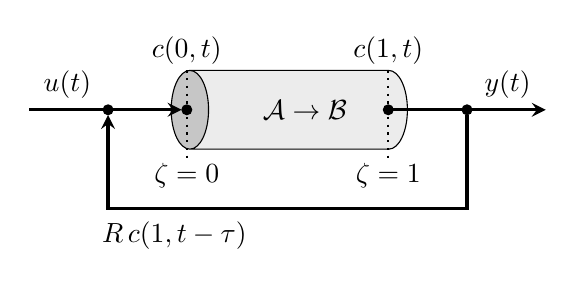
\begin{tikzpicture}
        \node (pfr) [cylinder, draw, minimum height=3cm, minimum width=1cm, shape aspect=1, shape border rotate=180, cylinder uses custom fill, cylinder end fill=gray!45, cylinder body fill=gray!15] {$\mathcal{A} \rightarrow \mathcal{B}$};
        \node (pfr_inlet) [circle, left of=pfr, xshift=-0.5cm, fill=black, draw, inner sep=0pt, minimum size=0.25cm, scale=0.5] {};
        \node (pfr_outlet) [circle, at={(pfr.east)}, shift={(-0.25cm,0)}, fill=black, draw, inner sep=0pt, minimum size=0.25cm, scale=0.5] {};
        \node (recycle_right) [circle, right of=pfr_outlet, fill=black, draw, inner sep=0pt, minimum size=0.25cm, scale=0.5] {};
        \node (recycle_left) [circle, left of=pfr_inlet, fill=black, draw, inner sep=0pt, minimum size=0.25cm, scale=0.5] {};
        
        \draw[dotted, thick] ([yshift=0.5cm]pfr_inlet.center) -- node[at end, below, yshift=0.1cm] {$\zeta = 0$} ([yshift=-0.65cm]pfr_inlet.center);
        \draw[dotted, thick] ([yshift=0.5cm]pfr_outlet.center) -- node[at end, below, yshift=0.1cm] {$\zeta = 1$} ([yshift=-0.65cm]pfr_outlet.center);
        
        \node[below of=recycle_left, node distance=1.3cm, anchor=north west, xshift=-0.2cm] {$R \, c(1, t-\tau)$};
        \node[above of=pfr_inlet, node distance=0.75cm,] {$c(0, t)$};
        \node[above of=pfr_outlet, node distance=0.75cm,] {$c(1, t)$};
        
        \draw [arrow_2] (pfr_outlet) -- node[near end, above] {$y(t)$} ++(2,0);
        \draw [arrow_2] (pfr_inlet) ++(-2,0) coordinate(start) -- node[near start, above] {$u(t)$} (pfr_inlet);
        \draw [arrow_2] (recycle_right) -- ++(0,-1.25) -| (recycle_left);
        
    \end{tikzpicture}
    \caption{Axial tubular reactor with recycle stream.}
    \label{fig:reactor_scheme}
    % \pdfbookmark[2]{Figure: Reactor Scheme}{fig:reactor_scheme}
\end{figure}

\begin{equation} \label{eq:PDE_original_model}
    \dot{c}(\zeta, t) = D \partial_{\zeta \zeta} c(\zeta, t) - v \partial_\zeta c(\zeta, t) + k_r c(\zeta, t)
\end{equation}

\begin{align} \label{eq:BC}
    \begin{cases}
        &D \partial_\zeta c(0, t) - v c(0, t) = -v \left[ R c(1, t-\tau) + (1-R) u(t) \right] \\
        &\partial_\zeta c(1, t) = 0 \\
        &y(t) = c(1, t)
    \end{cases}
\end{align}

Here, $c(\zeta, t)$ is the concentration of the product along the reactor, representing the state of the system. The physical parameters $D$, $v$, $k_r$, $R$, and $\tau$ represent the diffusion coefficient, flow velocity along the reactor, reaction constant, recycle ratio, and residence time of the recycle flow, respectively. The coordinate system in space and time is represented by $\zeta$ and $t$, where $\zeta \in [0, 1]$ and $t \in [0, \infty)$.

In an attempt to make the model more realistic for common axial dispersion tubular reactors in chemical industry, Dankwerts boundary conditions are chosen as they are known to be suitable for this purpose by accounting for deviations from perfect mixing and piston flow, assuming negligible transport lags in connecting lines \cite{danckwerts1993continuous}. The delayed state resulting from the recycled portion of the flow, occurring $\tau$ seconds back in time, is applied at the inlet boundary condition, as shown in (\ref{eq:BC}).

In the case where the problem involves similar forms of PDEs, an effective general practice to address delays in systems is to reformulate the problem such that the notion of delay is replaced with an alternative transport PDE. Therefore, a new state variable $\underline{x}(\zeta, t)$ is defined as a vector of functions $\equiv [x_1(\zeta, t), x_2(\zeta, t)]^T$, where $x_1(\zeta, t)$ represents the concentration within the reactor—analogous to $c(\zeta,t)$—and $x_2(\zeta, t)$ is introduced as a new state variable to account for the concentration along the recycle stream. The delay is thus modeled as a pure transport process, wherein the first state $x_1(\zeta, t)$ is transported from the reactor outlet to the inlet, experiencing a delay of $\tau$ time units while in the recycle stream. This makes all state variables expressed explicitly at a specific time instance $t$, resulting in the standard state-space form for a given infinite-dimensional linear time-invariant (LTI) system as $\dot{\underline{x}} = \mathfrak{A} \underline{x} + \mathfrak{B} u$. Here, $\mathfrak{A}$ is a linear operator $\mathcal{L}(X)$ acting on a Hilbert space $X: L^2[0,1] \times L^2[0,1]$ and $\underline{x}(\zeta,t)$, as defined previously, is the vector of functions describing the states of the system. The operator $\mathfrak{A}$ and its domain are defined in detail as shown in (\ref{eq:operator_A}). Also, $\mathfrak{B}$ is a linear operator that maps the scalar input from input-space onto the state space, as defined in (\ref{eq:operator_B}).

\begin{equation} \label{eq:operator_A}
    \begin{aligned}
        \mathfrak{A} \equiv&
        \begin{bmatrix}
            D \partial_{\zeta \zeta} - v \partial_\zeta + k_r & 0 \\
            0 & \frac{1}{\tau} \partial_\zeta
        \end{bmatrix}\\
        D(\mathfrak{A}) =& \Bigl\{ \underline{x}(\zeta) = [x_1(\zeta), x_2(\zeta)]^T \in X:\\
        &\underline{x}(\zeta), \partial_\zeta \underline{x}(\zeta), \partial_{\zeta \zeta} \underline{x}(\zeta) \quad \mathrm{a.c.},\\
        &D \partial_\zeta x_1(0) - v x_1(0) = -v R x_2(0),\\
        &\partial_\zeta x_1(1) = 0,
        x_1(1) = x_2(1) \Bigr\}
    \end{aligned}
\end{equation}

\begin{equation} \label{eq:operator_B}
    \begin{aligned}
        \mathfrak{B} &\equiv
        \begin{bmatrix}
            \delta(\zeta) \\
            0
        \end{bmatrix} v (1-R) \\
        D(\mathfrak{B}) &= \Bigl\{ u \in \mathbb{R} \Bigr\}
    \end{aligned}
\end{equation}

where $\delta(\zeta)$ is dirac delta function. This will enable the derivation of the system's spectrum using the eigenvalue problem. The characteristics equation of the system is obtained by solving the equation $det(\mathfrak{A}-\lambda_i~I)~=~0$ for $\lambda_i$, where $\lambda_i \in \mathbb{C}$ is the $i^{\text{th}}$ eigenvalue of the system and $I$ is the identity operator. Attempts to analytically solve this equation has failed; therefore, it is solved numerically using the parameters in Table~\ref{tab:pars}. The resulting eigenvalue distribution is depicted in Figure~\ref{fig:eigval_dist} in the complex plane.

\begin{figure}[!htbp]
    \centering
    \includesvg[inkscapelatex=false, width=0.35\textwidth, keepaspectratio]{Figures/eig_val_dist_R_0.3.svg}
    \caption{Eigenvalues of operator $\mathfrak{A}$.}
    \label{fig:eigval_dist}
\end{figure}


\begin{table}[ht]
    \centering
    \caption{Physical Parameters for the System}
    \label{tab:pars}
    \begin{tabular}{|c|c|c|c|}
    \hline
    \textbf{Parameter}        & \textbf{Symbol} & \textbf{Value}     & \textbf{Unit}    \\ \hline
    Diffusivity               & $D$             & $2\times10^{-5}$   & ${m^2}/{s}$      \\ \hline
    Velocity                  & $v$             & $0.01$   & ${m}/{s}$        \\ \hline
    Reaction Constant         & $k_r$           & $1.5$              & $s^{-1}$         \\ \hline
    Recycle Residence Time    & $\tau$          & $80$               & $s$              \\ \hline
    Recycle Ratio             & $R$             & $0.3$              & $-$              \\ \hline
    \end{tabular}
\end{table}

\subsection{Adjoint system}

Next step is to obtain the adjoint system operators $\mathfrak{A}^*$ and $\mathfrak{B}^*$. Utilizing the relation $\langle \mathfrak{A} \underline{x} + \mathfrak{B} u, \underline{y}\rangle = \langle \underline{x}, \mathfrak{A}^* \underline{y}\rangle + \langle u, \mathfrak{B}^* \underline{y}\rangle$, the adjoint operators $\mathfrak{A}^*$ and $\mathfrak{B}^*$ are obtained as shown in (\ref{eq:adjoint_A}) and (\ref{eq:adjoint_B}), respectively.


\begin{equation} \label{eq:adjoint_A}
    \begin{aligned}
        {\mathfrak{A}}^{*} =&
        \begin{bmatrix}
            D \partial_{\zeta \zeta} + v \partial_\zeta +k_r & 0\\
            0 & -\frac{1}{\tau} \partial_\zeta
        \end{bmatrix}\\
        D(\mathfrak{A}^*) =& \Bigl\{ \underline{y} = [y_1, y_2]^T \in Y:\\
        &\underline{y}(\zeta), \partial_\zeta \underline{y}(\zeta), \partial_{\zeta \zeta} \underline{y}(\zeta) \quad \mathrm{a.c.},\\
        &D \partial_\zeta y_1(1) + v y_1(1) = \frac{1}{\tau} y_2(1), \\
        &R v y_1(0) = \frac{1}{\tau} y_2(0), 
        \partial_\zeta y_1(0) = 0 \Bigr\}
    \end{aligned}
\end{equation}

\begin{equation} \label{eq:adjoint_B}
    \mathfrak{B}^* (\cdot) = \Bigl[ v(1-R) \int_0^1 \delta(\zeta) (\cdot) d\zeta \quad , \quad 0 \Bigr]
\end{equation}

Once the adjoint operators are determined, the eigenfunctions $\{ \underline{\phi_i}(\zeta), \underline{\psi_i}(\zeta) \}$ (for $\mathfrak{A}$ and $\mathfrak{A}^*$, respectively) may be obtained and properly scaled following the calculation of eigenvalues. The set of scaled eigenfunctions will then form a bi-orthonormal basis for the Hilbert space $X$; which will be later used in the controller design. It is important to note that the system is not self adjoint, as the obtained adjoint operator and its domain are not the same as the original operator and its domain.

\subsection{Resolvent operator}

One must obtain the resolvent operator of the system prior to constructing the discrete-time representation of the system. One way to represent the resolvent operator is by utilizing the modal characteristics of the system, resulting in an infinite-sum representation of the operator. While being a common practice in the literature, truncating the infinite-sum representation for numerical implementation may lead to a loss of accuracy. Another way to express the resolvent operator is by treating it as an operator that maps either the initial condition of the system $\underline{x}(\zeta,0)$ or the input $u(t)$, to the laplace transform of the state of the system $\underline{X}(\zeta, s)$. This approach, although more computationally intensive, results in a closed form expression for the resolvent operator, preserving the infinite-dimensional nature of the system. The resolvent operator $\mathfrak{R}(s, \mathfrak{A}) = (sI-\mathfrak{A})^{-1}$ is therefore obtained by applying laplace transform to the LTI representation of the system for both for zero-input response and zero-state response, and solving for $\underline{X}(\zeta, s)$.
% The procedure as well as the resulting closed form expression for the resolvent operator is shown in Appendix~\ref{app:resolvent}.

Since the system generator $\mathfrak{A}$ is not self-adjoint, the resolvent operator for the adjoint system shall also be obtained. This is done in a similar manner as the original system, resulting in a closed-form expression for the adjoint resolvent operator $\mathfrak{R}^*(s, \mathfrak{A}^*)$.
% as shown in Appendix~\ref{app:resolvent}.

\subsection{Caley-Tustin time discretization}

Having access to the resolvent operators of the original and the adjoint system, the Caley-Tustin time-discretization may be utilized to map the continuous-time setting to the discrete-time setting without losing crucial dynamical properties of the system, such as stability and controllability. This Crank-Nicolson type of discretization is also known as the lowest order symplectic integrator in Gauss quadrature-based Runge-Kutta methods \cite{hairer2006geometric}. Considering $\Delta t$ as the sampling time, and assuming a piecewise constant input within time intervals (a.k.a. zero-order hold), the discrete-time representation $\underline{x}(\zeta, k) = \mathfrak{A}_d \underline{x}(\zeta, k-1) + \mathfrak{B}_d u(k)$ is obtained, with discrete-time operators $\mathfrak{A}_d$ and $\mathfrak{B}_d$ defined in (\ref{eq:discrete_AB}), where $\alpha = 2/{\Delta t}$.

\begin{equation} \label{eq:discrete_AB}
    \begin{bmatrix}
        \mathfrak{A}_d & \mathfrak{B}_d
    \end{bmatrix} = 
    \begin{bmatrix}
        -I + 2\alpha \mathfrak{R}(\alpha, \mathfrak{A}) & \sqrt{2\alpha} \mathfrak{R}(\alpha, \mathfrak{A}) \mathfrak{B}
    \end{bmatrix}
\end{equation}

As required for systems with nonself-adjoint generators, the adjoint discrete-time operators $\mathfrak{A}_d^*$ and $\mathfrak{B}_d^*$ are also obtained in a similar manner, as shown in (\ref{eq:discrete_AB_star}).

\begin{equation} \label{eq:discrete_AB_star}
    \begin{bmatrix}
        \mathfrak{A}_d^* & \mathfrak{B}_d^*
    \end{bmatrix} = 
    \begin{bmatrix}
        -I + 2\alpha \mathfrak{R}^*(\alpha, \mathfrak{A}^*) & \sqrt{2\alpha} \mathfrak{B}^* \mathfrak{R}^*(\alpha, \mathfrak{A}^*)
    \end{bmatrix}
\end{equation}

\subsection{Model predictive control design}

The proposed MPC, as shown in Fig.~\ref{fig:block_diagram}, is developed in this section with the goal of stabilizing the given unstable infinite-dimensional system within an optimal framework while satisfying input constraints. An infinite-time open-loop objective function sets the foundation of the controller design in the discrete-time setting at each sampling instant $k$, which consists of a weighted sum of state deviations and actuation costs for all future time instances, subject to the system dynamics and input constraints, as shown in (\ref{eq:MPC_inf_time}).

\begin{figure}[!htbp]
    \centering
    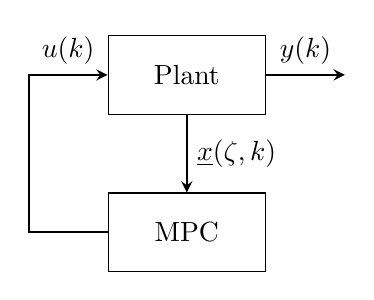
\begin{tikzpicture}[node distance=2cm]
        \node (plant) [block] {Plant};
        \node (MPC) [block, below of=plant] {MPC};
        \draw [arrow] (plant.south) -- node[midway, right] {$\underline{x}(\zeta,k)$} (MPC.north);
        \draw [arrow] (MPC.west) -- ++(-1,0) |- node[near end, above] {$u(k)$} (plant.west);
        \draw [arrow] (plant.east) -- node[midway, above] {$y(k)$} ++(1,0);
    \end{tikzpicture}
    \caption{Proposed full-state feedback model predictive control system.}
    \label{fig:block_diagram}
\end{figure}

\begin{equation} \label{eq:MPC_inf_time}
    \begin{aligned}
        \min_{U} \quad \sum_{l=0}^{\infty} &\langle \underline{x}(\zeta, k+l | k), \mathfrak{Q} \underline{x}(\zeta, k+l | k) \rangle \\
        + &\langle u(k+l+1 | k), \mathfrak{F} u(k+l+1|l) \rangle \\
        \, \\
        \text{s.t.} \quad &\underline{x}(\zeta, k+l | k) = \mathfrak{A}_d \underline{x}(\zeta, k+l-1 | k) + \mathfrak{B}_d u(k+l | k) \\
        &u^{min} \leq u(k+l | k) \leq u^{max}
    \end{aligned}
\end{equation}

where $\mathfrak{Q}$ and $\mathfrak{F}$ are positive definite operators of appropriate dimensions, responsible for penalizing state deviations and actuation costs, respectively. The notation $(k+l|k)$ indicates the future time states or input instance $k+l$ obtained at time $k$. The infinite-time optimization problem may be reduced to a finite-time setup by assigning zero-input beyond a certain control horizon $N$, result in the optimization problem in (\ref{eq:MPC_finite_time}).

\begin{equation} \label{eq:MPC_finite_time}
    \begin{aligned}
        \min_{U} \quad \sum_{l=0}^{N-1} &\langle \underline{x}(\zeta, k+l | k), \mathfrak{Q} \underline{x}(\zeta, k+l | k) \rangle \\
        + &\langle u(k+l+1 | k), \mathfrak{F} u(k+l+1|l) \rangle \\
        + &\langle \underline{x}(\zeta, k+N | k), \mathfrak{P} \underline{x}(\zeta, k+N | k) \rangle \\
        \, \\
        \text{s.t.} \quad &\underline{x}(\zeta, k+l | k) = \mathfrak{A}_d \underline{x}(\zeta, k+l-1 | k) + \mathfrak{B}_d u(k+l | k) \\
        &u^{min} \leq u(k+l | k) \leq u^{max} \\
        & \langle \underline{x}(\zeta, k+N | k), \underline{\phi_u}(\zeta) \rangle = 0
    \end{aligned}
\end{equation}

Obtained as the solution to the discrete-time Lyapunov equation, $\mathfrak{P}$ is the terminal cost operator as shown in (\ref{eq:terminal_cost}); which can be proven to be positive definite only if the terminal state $\underline{x}(\zeta, k+N | k)$ is in a stable subspace. Therefore, an equality constraint is introduced to guarantee that the resulting quadratic optimization problem is convex. The terminal constraint is enforced by setting the projection of the terminal state onto the unstable subspace of the system to zero \cite{curtainbook, xu2017linear, khatibi2021model}. Here, $\underline{\phi_u}(\zeta)$ is the set of unstable eigenfunctions of the system, for all eigenvalues where $\operatorname{Re}(\lambda_u) \geq 0$.

\begin{equation} \label{eq:terminal_cost}
    \mathfrak{P} (\cdot) = \sum_{m=0}^{\infty} \sum_{n=0}^{\infty} 
    -\frac{
        \langle \underline{\phi_m} , \mathfrak{Q} \underline{\psi_n} \rangle
    }{
        \lambda_m + \overline{\lambda_n}
    }
    \langle (\cdot) , \underline{\psi_n} \rangle \phi_m
\end{equation}

One may further process the optimization problem in (\ref{eq:MPC_finite_time}) to obtain a standard format for quadratic programming (QP) solvers by substituting the future states in terms of the current state and the sequence of future inputs using system dynamics expression. The resulting QP problem is given in (\ref{eq:MPC_QP}). The optimal input sequence $U$ is then obtained by solving the QP problem at each sampling instant $k$. To implement a receding horizon control strategy, only the first input of the optimal sequence $u(k|k)$ is applied to the system, and the optimization problem is solved again at the next sampling instant $k+1$.

\begin{equation} \label{eq:MPC_QP}
    \begin{aligned}
        \min_{U} &J = U^T \langle I,H \rangle U + 2U^T \langle I, P \underline{x}(\zeta, k|k) \rangle \\
        \text{s.t.} &\qquad U^{min} \leq U \leq U^{max} \\
        &\qquad T_u \underline{x}(\zeta, k|k) + S_u U = 0
        \, \\
        \text{with } &H = \\
        &\hspace{-3.5em }\begin{bmatrix}
            \mathfrak{B}_d^* \mathfrak{P} \mathfrak{B}_d + \mathfrak{F} & \mathfrak{B}_d^* \mathfrak{A}_d^* \mathfrak{P} \mathfrak{B}_d & \cdots &  \mathfrak{B}_d^* {\mathfrak{A}_d^*}^{N-1} \mathfrak{P} \mathfrak{B}_d \\
            \mathfrak{B}_d^* \mathfrak{P} \mathfrak{A}_d \mathfrak{B}_d & \mathfrak{B}_d^* \mathfrak{P} \mathfrak{B}_d + \mathfrak{F} & \cdots & \mathfrak{B}_d^* {\mathfrak{A}_d^*}^{N-2} \mathfrak{P} \mathfrak{B}_d \\
            \vdots & \vdots & \ddots & \vdots \\
            \mathfrak{B}_d^* \mathfrak{P} {\mathfrak{A}_d}^{N-1} \mathfrak{B}_d & \mathfrak{B}_d^* \mathfrak{P} {\mathfrak{A}_d}^{N-2} \mathfrak{B}_d & \cdots & \mathfrak{B}_d^* \mathfrak{P} \mathfrak{B}_d + \mathfrak{F}
        \end{bmatrix} \\
        P = &\begin{bmatrix}
            \mathfrak{B}_d^* \mathfrak{P} {\mathfrak{A}_d} &
            \mathfrak{B}_d^* \mathfrak{P} {\mathfrak{A}_d}^{2}  &
            \hdots &
            \mathfrak{B}_d^* \mathfrak{P} {\mathfrak{A}_d}^{N} 
        \end{bmatrix}^T \\
        T_u (\cdot) = &\begin{bmatrix}
            \langle {\mathfrak{A}_d}^{N} (\cdot), \underline{\phi_u} \rangle
        \end{bmatrix} \\
        S_u = &\begin{bmatrix}
            \langle {\mathfrak{A}_d}^{N-1} \mathfrak{B}_d, \underline{\phi_u} \rangle & 
            \langle {\mathfrak{A}_d}^{N-2} \mathfrak{B}_d, \underline{\phi_u} \rangle &
            \hdots &
            \langle \mathfrak{B}_d, \underline{\phi_u} \rangle
        \end{bmatrix} \\
        U = &\begin{bmatrix}
            u(k+1|k) & u(k+2|k) & \hdots & u(k+N|k)
        \end{bmatrix}^T
    \end{aligned}
\end{equation}
\section{Results and Discussion}

Numerical simulations for the open-loop system and the closed-loop system under the proposed MPC are presented in this section, with parameters chosen according to Table~\ref{tab:pars}. As the eigenvalue distribution obtained in Fig(\ref{fig:eigval_dist}) suggests, the open-loop system is unstable due to the presence of an eigenvalue with positive real part. The zero-input response of the system is shown in Fig(\ref{fig:openloop_response}) where the initial condition for the reactor is set to $c(\zeta,0) = \sin^2(\pi \zeta)$. The recycle stream is assumed to be empty at the beginning of the simulation.

\begin{figure}[!htbp]
    \centering
    \includesvg[inkscapelatex=false, width=0.4\textwidth, keepaspectratio]{Figures/openloop_response.svg}
    \caption{Open-loop concentration profile along the reactor.}
    \label{fig:openloop_response}
\end{figure}

An infinite-dimensional MPC is designed and applied to the unstable system. The state deviation and actuation penalty terms are set as $\mathfrak{Q} = 0.04 I$ and $\mathfrak{F} = 27$. The sampling time and the horizon length for the MPC are set to $\Delta t = 20$ s and $N = 9$, respectively. Lastly, the input constraints are assumed to be $0 \leq u(t) \leq 0.15$. The closed-loop response of the system is shown in Fig(\ref{fig:closedloop_response}) and the control input as well as the system output is shown in Fig(\ref{fig:control_input}). It may be confirmed that the MPC successfully stabilizes the unstable system while satisfying the input constraints.

\begin{figure}[!htbp]
    \centering
    \includesvg[inkscapelatex=false, width=0.4\textwidth, keepaspectratio]{Figures/closedloop_response.svg}
    \caption{Stabilized reactor concentration profile under the proposed MPC.}
    \label{fig:closedloop_response}
\end{figure}

\begin{figure}[!htbp]
    \centering
    \includesvg[inkscapelatex=false, width=0.4\textwidth, keepaspectratio]{Figures/input.svg}
    \caption{Input constraints, the obtained input profile, and the reactor output under the proposed MPC.}
    \label{fig:control_input}
\end{figure}

One interesting aspect of considering recycle stream is the oscillatory behavior of the system dynamics. While axial dispersion reactors show no oscillation in the absence of recycle, the nature of recycle streams can introduce such behavior. The choice of control horizon is another key factor. A short control horizon relative to the resident time of the recycle stream can lead to oscillatory input profiles due to the presence of delayed recycle stream. In this example, the control horizon, i.e. $180$ s, is set to be considerably longer than the recycle delay, which is $80$ s; resulting in a non-oscillatory input profile.
\section{Conclusion}
\section*{Acknowledgment}

% Include the bibliography
\bibliographystyle{IEEEtran}
\bibliography{./IEEEabrv,./references}  % Include both abbreviation and reference files




\end{document}
